%%% Local Variables:
%%% mode: latex
%%% TeX-master: t
%%% End:

\documentclass{article}

\usepackage{amsmath}
\usepackage{amssymb}
\usepackage{minted}
\usepackage{graphicx}

\graphicspath{ {images/} }

\title{Modern Statistical Methods Assignment}
\author{James Aley}
\date{February 2016}

\begin{document}

\maketitle

\section*{Question 1}

\subsection*{(a)}

The Pareto distribution has probability density function $f(x)$ given by:

\begin{displaymath}
  f(x) = \frac{\alpha \beta^{\alpha}}{{(x + \beta)}^{\alpha + 1}} \quad x \geq 0
\end{displaymath}

To calculate the cumulative distribution function, we integrate this
function over the support \(x \geq 0\):

%% &= \left[   \right]_0^\infty

\begin{align*}
  F(u) &= \int_0^u f(x) \, \mathrm{d}x \\
       &= \int_0^u \frac{\alpha \beta^{\alpha}}
                            {{(x + \beta)}^{\alpha + 1}}
         \, \mathrm{d}x \\
       &= {\left[ - \beta^\alpha {(x + \beta)}^{-\alpha}  \right]}_0^u \\
       &= 1 - \frac{\beta^{\alpha}}{{(u + \beta)}^\alpha} \\
       &= 1 - {\left( \frac{\beta}{u + \beta} \right)}^{\alpha}
\end{align*}

Now, to calculate the expected value, using integration by parts:

\begin{align*}
  \mathbf{E}\left[X\right] &= \int_0^{\infty} x f(x) \mathrm{d}x \\
                           &= \int_0^{\infty} \frac{x \alpha \beta^{\alpha}}
                             {{(x + \beta)}^{\alpha + 1}}
                             \, \mathrm{d}x \\
                           &= {\left[
                             - \beta^\alpha x {(x + \beta)}^{-\alpha}
                             + \int \beta^{\alpha} {(x + \beta)}^{- \alpha}
                             \right]}_0^{\infty} \\
                           &= {\left[
                             - \beta^\alpha x {(x + \beta)}^{-\alpha}
                             + \frac{\beta^{\alpha}}{1 - \alpha}
                             {\left( x + \beta \right)}^{1 - \alpha}
                             \right]}_0^{\infty} \\
\end{align*}

We can see by taking limits on the upper bounds, that we require
$\alpha > 1$ in order for this integral to converge.

\begin{align*}
  \lim_{x \to \infty} {\left[
  - \beta^\alpha x {(x + \beta)}^{-\alpha}
  + \frac{\beta^{\alpha}}{1 - \alpha}
  {\left( x + \beta \right)}^{1 - \alpha}
  \right]}_0^{\infty} = 0
  \quad \left(  \alpha > 1 \right)
\end{align*}

Therefore, substituting in $x = 0$ and subtracting from $0$ gives us:

\begin{align*}
  \mathbf{E}\left[X\right] &= 0 - \frac{\beta^\alpha}{\beta^\alpha}
                             \left( \frac{\beta}{1 - \alpha}
                             \right) \\
                           &= \frac{\beta}{\alpha - 1}
\end{align*}

For the median, we need to find the value $m$ that puts equal
probability density on either side of it. That is to say that $F(x) =
\frac{1}{2}$

\begin{align*}
  F(m) &= \frac{1}{2} \\
  1 - {\left( \frac{\beta}{m + \beta} \right)}^{\alpha} &= \frac{1}{2} \\
  \frac{\beta}{m + \beta} &= {\frac{1}{2}}^{\frac{1}{\alpha}} \\
  m &= \beta \left( \frac{1}{2^{\frac{1}{\alpha}}} - 1 \right)
\end{align*}

To calculate the variance, $\mathbf{Var}\left[ X \right]$, we shall
make use of the formula:

\[
  \mathbf{Var}\left[ X \right] = \mathbf{E}\left[X^2\right]
  - {\mathbf{E}\left[X\right]}^2
\]

We already have the first moment available from from calculating the
mean earlier, so now we need to calculate the second moment,
$\mathbf{E}\left[X^2\right]$ as follows. This time, we'll need to
apply integration by parts twice successively.

\begin{align*}
  \mathbf{E}\left[X^2\right] &= \int_0^{\infty}
                               x^2 f(x) \, \mathrm{d}x \\
                             &= \int_0^{\infty}
                               \frac{x^2 \alpha \beta^\alpha}
                               {{\left( x + \beta \right)}^{\alpha +
                               1}} \, \mathrm{d}x \\
                             &= \alpha \beta^\alpha
                               {\left[
                               \frac{-x^2
                               {\left( x + \beta \right)}^{- \alpha}}
                               {\alpha}
                               - \int \frac{-2x{(x + \beta)}^{- \alpha}}
                               {\alpha}
                               \right]}_0^{\infty} \\
                             &= \beta^\alpha
                               {\left[
                               -x^2 {(x + \beta)}^{-\alpha}
                               + \left(
                               \frac{2x{\left(x + \beta \right)}^{1 - \alpha}}
                               {(1 - \alpha)}
                               - \int \frac{2{\left( x + \beta
                               \right)}^{1 - \alpha}}
                               {(1 - \alpha)}
                               \right)
                               \right]}_0^{\infty} \\
                             &= \beta^\alpha
                               {\left[
                               -x^2 {(x + \beta)}^{-\alpha}
                               + \frac{2x{\left(x + \beta \right)}^{1 - \alpha}}
                                 {(1 - \alpha)}
                               + \frac{2 {\left(x + \beta \right)}^{2 - \alpha}}
                                 {(1 - \alpha)(2 - \alpha)}
                               \right]}_0^{\infty}
\end{align*}

This integral will only converge if we require that $\alpha > 2$, in
which case we take limits for $x$ as before:

\begin{displaymath}
\lim_{x \to \infty}
\beta^\alpha
  {\left[
  -x^2 {(x + \beta)}^{-\alpha}
  + \frac{2x{\left(x + \beta \right)}^{1 - \alpha}}
  {(1 - \alpha)}
  + \frac{2 {\left(x + \beta \right)}^{2 - \alpha}}
  {(1 - \alpha)(2 - \alpha)}
  \right]}
= 0
\end{displaymath}

Note that the requirement that $\alpha > 2$ is important both so that
the $x^2$ component above grows more slowly than the denominator, and
so that the final quotient is finite. Again, we substitute in $x = 0$
and subtract from the $0$ obtained from this limit to get an
expression for the second moment:

\begin{align*}
  \mathbf{E}\left[X^2\right] &= 0 - \beta^{\alpha} \left(
                               \frac{2 \beta^{2 - \alpha}}
                               {(1 - \alpha)(2 - \alpha)}
                               \right) \\
                             &= \frac{2 \beta^2}
                               {(\alpha - 1)(\alpha - 2)}
\end{align*}

Returning to the expression for $\mathbf{Var}\left[ X \right]$, we have:

\begin{align*}
  \mathbf{Var}\left[ X \right] &= \mathbf{E}\left[X^2\right]
                                 - {\mathbf{E}\left[X\right]}^2 \\
                               &= \frac{2 \beta^2}
                                 {(\alpha - 1)(\alpha - 2)}
                                 - {\left(
                                 \frac{\beta}{\alpha - 1}
                                 \right)}^2 \\
                               &= \frac{2 \beta^2 \alpha (\alpha - 1)
                                 - \beta^2 (\alpha - 2)}
                                 {{(\alpha - 1)}^2(\alpha - 2)} \\
                               &= \frac{\beta^2 \alpha}
                                 {{(\alpha - 1)}^2(\alpha - 2)}
\end{align*}

\subsection*{(b)}

To generate samples from the Pareto distribution, using uniform
variables, we can invert the CDF obtained in the previous section as
follows.

\begin{align*}
  F(x) &= 1 - {\left( \frac{\beta}{x + \beta} \right)}^\alpha \\
  \frac{\beta}{x + \beta} &= {\left( 1 - F(x) \right)}^{\frac{1}{\alpha}} \\
                        x &= \beta \left[{ \left( 1 - F(x)
                            \right)}^{-\frac{1}{\alpha}} - 1 \right]
\end{align*}

This gives us an expression for $F^{-1}(x)$, the inverse cumulative
distribution function:

\[
  F^{-1}(u) = \beta \left[{ \left( 1 - u \right)}^{-\frac{1}{\alpha}}
    - 1 \right]
\]

We may now use values for $u$, which should be realisations of  $U
\sim \mathrm{Uniform}(0, 1)$. These may be generated using a
congruential generator, or any standard method for generating
pseudo-random uniform numbers. The \texttt{runif()} function can be
used to achieve this in R.

\subsection*{(c)}

The following code snippet includes implementations of the Pareto
distribution PDF, CDF and inverse CDF, as calculated in the previous
section. Following those function definitions, we make use of them to
simulate values from the Pareto distribution and visualise that
simulation using the method outlined previously.

\begin{minted}{R}
#' Probability density function for the Paretro distribution, with
#' parameters alpha and beta
pareto.pdf <- function(alpha, beta, x) {
  (alpha * beta^alpha) / (x + beta)^(alpha + 1)
}

#' Cumulative distribution funtion for Paretro distribution with paremeters
#' alpha abd beta.
pareto.cdf <- function(alpha, beta, u) {
  1 - (beta / (u + beta))^alpha
}

#' Inverse cumulative distribution function for the Pareto
#' distribution. Alpha and Beta are distribution parameters,
#' q should be a value between 0 and 1.
pareto.inv.cdf <- function(alpha, beta, q) {
  beta * ((1 - q)^(-1/alpha) - 1)
}

## Compare simulated values to the density function
require(ggplot2)

pareto <- data.frame(simulated = pareto.inv.cdf(3, 100000, runif(10000)))

ggplot(pareto, aes(simulated)) +
  geom_density(colour="red", fill="red", alpha=0.1) +
  stat_function(fun = function(x) {pareto.pdf(3, 100000, x)},
                colour="blue", geom="area", alpha=0.1, fill="blue") +
  xlab("X") +
  ylab("Density") +
  xlim(0, 100000)
\end{minted}

Note that in Figure \ref{fig:q1c_histogram} we're plotting the real
Pareto PDF against the \emph{density} of the simulated values, so that
they are on comparable scales. We're also focusing on the range for
$X$ in 0 to 100,000, before entering the very long tail. We can see
that the simulation fits the PDF reasonably well, and is mostly unable
to reach the very low extremes of the real PDF.

\begin{figure}
  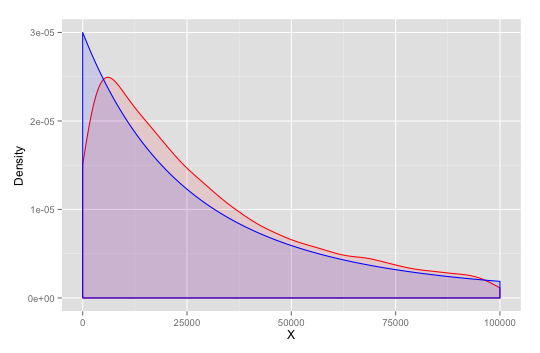
\includegraphics[width=\textwidth]{q1c_histogram}
  \caption{Simulated value density (red) plotted against exact Pareto
    PDF (blue).}
  \centering
  \label{fig:q1c_histogram}
\end{figure}

\subsection*{(d)}

Insurance claims are likely to me well-modeled by the Pareto
distribution, as it is very heavy-tailed. It is able to realistically
represent the very low probability of large claims, corresponding to
extreme loss for the insurer. Insurance claims are also likely to
follow the \emph{Pareto Principle}, in that most of the value of the
payments made will be to relatively few (large) claims.

\section*{Question 2}

The following R code snippet simulates possible outcomes for 1000
customers, each with a claim probability of 0.1 in a year. We assume
the claims $X$ have distriubtion $X \sim \mathrm{Pareto}(3, 100000)$
as before.

We also note, given the restriction that each customer can only make a
single claim in a year, we essentially have a Bernoulli outcome variable
for whether or not each customer makes a claim with parameter $p =
0.1$. Modeling the event of a claim occurring as $1$ and not occurring
as $0$, we can extend this to $n$ customers be using a Binomial
distribution. If we let $N$ represent the number of claims, then:

\[
  N \sim \mathrm{Bin}(1000, 0.1)
\]

The code below uses this to model the number of claims,
\texttt{n\_claims} in each simulation iteration. That variable tells us
the number of uniform variables to draw and pass on to our inverse
Pareto CDF derived previously to model the value of claims for one year.

\begin{minted}{R}
#' Returns a vector of length n_runs containing simulated values
#' for the year end assets.
simulate.year.end.assets <- function(n_runs = 10000,
                                     start_assets = 250000,
                                     n_customers = 1000,
                                     premium = 6000,
                                     claim_prob = 0.1) {
  # Accumulate year-end assets in a vector
  outcomes <- numeric(length = n_runs)
  for(i in 1:n_runs) {
    # Number of claims this year, in this simulation
    n_claims <- rbinom(1, n_customers, claim_prob)

    # Calculate year-end profit/loss for this number of claims, by
    # drawing from Pareto distribution
    outcomes[i] <- start_assets +
      (n_customers * premium) -
      sum(pareto.inv.cdf(3, 100000, runif(n_claims)))
  }
  return(outcomes)
}

# Reformat simulation data into a data frame for plotting
# a histogram of the simulation outcomes
bankruptcy <- data.frame(assets=simulate.year.end.assets())
ggplot(bankruptcy, aes(assets)) +
  geom_density(colour="blue", fill="blue", alpha=0.1) +
  geom_vline(xintercept = 0, linetype="longdash") +
  xlab("Assets at Year End") +
  ylab("Probability Density")

# Calculate the probability of bankruptcy, i.e. the proportion
# of outcomes where year end profits were less than zero.
sum(bankruptcy['assets'] < 0) / n_runs
\end{minted}

In one simulation, we see a probability of bankruptcy probability of
0.0954, from the outcome distribution shown in Figure
\ref{fig:q2_histogram}.

\begin{figure}
  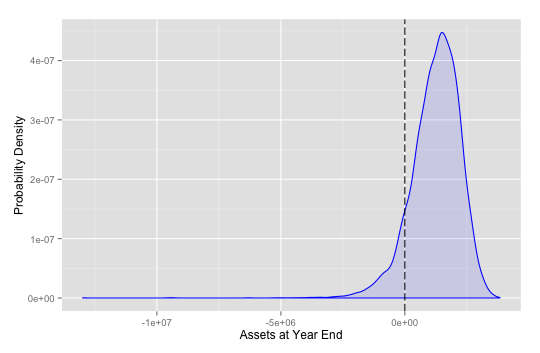
\includegraphics[width=\textwidth]{q2_histogram}
  \caption{Simulated year-end profit or loss.}
  \centering
\label{fig:q2_histogram}
\end{figure}

\section*{Question 3}

\subsection*{(a)}

The following code snippet makes use of the simulation function we
defined in the previous section, calling it with a different premium
price parameter many times to produce the plot in Figure~\ref{fig:q3_premiums}.

\begin{minted}{R}
#' Esimate the probability of bankruptcy for a premium of given price
bankruptcy.prob <- function(premium) {
  N <- 10000
  assets <- simulate.year.end.assets(premium=premium, n_runs=N)
  sum(assets < 0) / N
}

premiums <- seq(from=5500, to=8000, by=250)
premium.data <- data.frame(premium.price = premiums,
                           bankruptcy.prob = sapply(premiums, bankruptcy.prob))


ggplot(premium.data, aes(x=premium.price, y=bankruptcy.prob)) +
  geom_line(colour="blue") +
  stat_hline(yintercept = 0.02, linetype="longdash") +
  xlab("Premium Price (GBP)") +
  ylab("Probability of Bankruptcy")
\end{minted}

\begin{figure}
  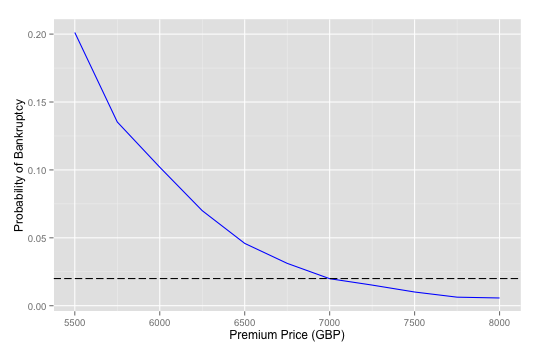
\includegraphics[width=\textwidth]{q3_premiums}
  \caption{Probability of bankruptcy for changing premium prices.}
  \centering
\label{fig:q3_premiums}
\end{figure}

As indicated by the dashed line in Figure~\ref{fig:q3_premiums}, we
should set the premium to \pounds{7000} or higher in order to see a probability
of bankruptcy below 2\%.

\subsection*{(b)}

Again, making use of the simulation functions defined previously, the
following code snippet reruns the simulation for varying claim
probabilities to produce the plot shown in Figure~\ref{fig:q3_claims}.

\begin{minted}{R}
bankruptcy.prob.claim <- function(claim.prob) {
  N <- 10000
  assets <- simulate.year.end.assets(claim_prob = claim.prob, n_runs=N)
  sum(assets < 0) / N
}

claims <- seq(from=0.05, to=0.15, by=0.005)
claim.data <- data.frame(claim.prob = claims,
                         bankruptcy.prob =
                           sapply(claims, bankruptcy.prob.claim))

ggplot(claim.data, aes(x=claim.prob, y=bankruptcy.prob)) +
  geom_line(colour="blue") +
  stat_hline(yintercept = 0.02, linetype="longdash") +
  xlab("Claim Probability") +
  ylab("Probability of Bankruptcy")
\end{minted}

Holding the premium price fixed at \pounds{6000}, as per the original
specification, we can see from Figure~\ref{fig:q3_claims} that the
company can only expect a bankruptcy probability below 2\% if the
claim probability is below 0.08.

\begin{figure}
  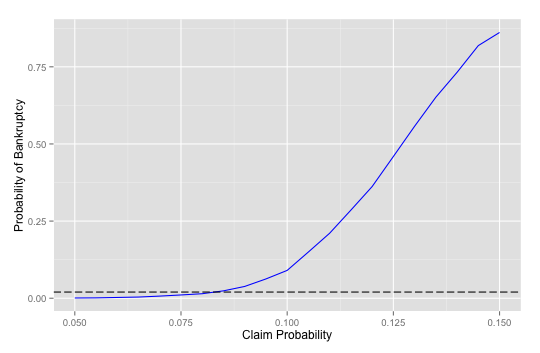
\includegraphics[width=\textwidth]{q3_claims}
  \caption{Bankruptcy probability for varying customer claim
    probabilities.}
  \centering
\label{fig:q3_claims}
\end{figure}



\end{document}
